\newcommand{\malwareResultsAucTable}{
	\begin{table}[H]
		\centering
		\begin{tabular}{|p{2,8cm}||p{2,8cm} p{2,8cm} p{2,8cm}|}
			\hline
			Malware Label & ALOHA & Joint Embedding & Proposed Model \\
			\hline
			AUC-ROC & \textBF{0.994$\pm$0.000} & - & \textBF{0.994$\pm$0.000} \\
			\hline
		\end{tabular}
		\caption{AUC-ROC (Area Under Curve) of the different models for the Malware Label prediction task. Best results are shown in \textbf{bold}.} \label{tab:malware_auc}
	\end{table}
}

\newcommand{\malwareResultsAtFprTable}{
	\begin{center}
		\begin{longtable}[c]{|p{3,2cm}||p{1,8cm} p{1,8cm} p{1,8cm} p{1,8cm} p{1,8cm}|}
			\hline
			Malware Label & \multicolumn{5}{c|}{{FPR}} \\
			& $10^{-5}$ & $10^{-4}$ & $10^{-3}$ & $10^{-2}$ & $10^{-1}$ \\
			\hline
			\endfirsthead
			
			\caption*{\raggedright ...continued from previous page} \\
			\hline
			Malware Label & \multicolumn{5}{c|}{\textbf{FPR}} \\
			& $10^{-5}$ & $10^{-4}$ & $10^{-3}$ & $10^{-2}$ & $10^{-1}$ \\
			\hline
			\endhead
			
			\caption*{\raggedleft ...continued on next page} \\
			\endfoot
			
			\caption{Mean and standard deviation results (TPR, Accuracy, Recall, Precision and F1-Score) of the different models for the Malware Label prediction task at different \textbf{FPR}s (\textit{False Positive Rates}). Best results are shown in \textbf{bold}. Under \textbf{TPR} results, it is presented also the mean detection error percentage reduction introduced by the \textit{Proposed Model} with respect to both \textit{ALOHA} model and \textit{Joint Embedding}.} \\
			\endlastfoot
			
			\multicolumn{6}{|c|}{\textbf{TPR}} \\
			\hline
			ALOHA & 0.478$\pm$0.000 & 0.746$\pm$0.000 & 0.885$\pm$0.000 & 0.955$\pm$0.000 & \textBF{0.987$\pm$0.000} \\
			Joint Embedding & - & - & - & - & - \\
			Proposed Model & \textBF{0.524$\pm$0.000} & \textBF{0.752$\pm$0.000} & \textBF{0.889$\pm$0.000} & \textBF{0.956$\pm$0.000} & \textBF{0.987$\pm$0.000} \\
			\hline
			Error Reduction wrt \newline ALOHA & 8.8\% & 2.4\% & 3.5\% & 2.2\% & 0.0\% \\
			Error Reduction wrt \newline Joint Embedding & - & - & - & - & - \\
			\hline
			\multicolumn{6}{|c|}{\textbf{Accuracy}} \\
			\hline
			ALOHA & 0.798$\pm$0.000 & 0.902$\pm$0.000 & 0.955$\pm$0.000 & \textBF{0.977$\pm$0.000} & \textBF{0.934$\pm$0.000} \\
			Joint Embedding & - & - & - & - & - \\
			Proposed Model & \textBF{0.816$\pm$0.000} & \textBF{0.904$\pm$0.000} & \textBF{0.957$\pm$0.000} & \textBF{0.977$\pm$0.000} & \textBF{0.934$\pm$0.000} \\
			\hline
			\multicolumn{6}{|c|}{\textbf{Recall}} \\
			\hline
			ALOHA & 0.478$\pm$0.000 & 0.746$\pm$0.000 & 0.885$\pm$0.000 & 0.955$\pm$0.000 & \textBF{0.987$\pm$0.000} \\
			Joint Embedding & - & - & - & - & - \\
			Proposed Model & \textBF{0.524$\pm$0.000} & \textBF{0.752$\pm$0.000} & \textBF{0.889$\pm$0.000} & \textBF{0.956$\pm$0.000} & \textBF{0.987$\pm$0.000} \\
			\hline
			\multicolumn{6}{|c|}{\textbf{Precision}} \\
			\hline
			ALOHA & \textBF{1.000$\pm$0.000} & \textBF{1.000$\pm$0.000} & \textBF{0.998$\pm$0.000} & \textBF{0.984$\pm$0.000} & \textBF{0.862$\pm$0.000} \\
			Joint Embedding & - & - & - & - & - \\
			Proposed Model & \textBF{1.000$\pm$0.000} & \textBF{1.000$\pm$0.000} & \textBF{0.998$\pm$0.000} & \textBF{0.984$\pm$0.000} & \textBF{0.862$\pm$0.000} \\
			\hline
			\multicolumn{6}{|c|}{\textbf{F1 Score}} \\
			\hline
			ALOHA & 0.646$\pm$0.000 & 0.855$\pm$0.000 & 0.938$\pm$0.000 & \textBF{0.969$\pm$0.000} & \textBF{0.920$\pm$0.000} \\
			Joint Embedding & - & - & - & - & - \\
			Proposed Model & \textBF{0.688$\pm$0.000} & \textBF{0.859$\pm$0.000} & \textBF{0.941$\pm$0.000} & \textBF{0.969$\pm$0.000} & \textBF{0.920$\pm$0.000} \\
			\hline
		\end{longtable}
	\end{center}
}

\newcommand{\malwareResultsSummaryTable}{
	\begin{table}[H]
		\centering
		\begin{tabular}{|p{3,2cm}||p{1,8cm} p{1,8cm} p{1,8cm} p{1,8cm} p{1,8cm}|}
			\hline
			\multicolumn{6}{|c|}{Malware label (at FPR $=1\%$)} \\
			\hline
			Model & TPR & Accuracy & Precision & Recall & F1 score \\
			\hline
			ALOHA & 0,955$\pm$0.000 & \textBF{0,977$\pm$0.000} & \textBF{0,984$\pm$0.000} & 0,955$\pm$0.000 & \textBF{0,969$\pm$0.000} \\
			Joint Embedding & - & - & - & - & - \\
			Proposed Model & \textBF{0,956$\pm$0.000} & \textBF{0,977$\pm$0.000} & \textBF{0,984$\pm$0.000} & \textBF{0,956$\pm$0.000} & \textBF{0,969$\pm$0.000} \\
			\hline
		\end{tabular}
		\caption{Summary of the mean and standard deviation results of the different models for the Malware Label prediction task at \textbf{FPR} $=1\%$. Best results are shown in \textbf{bold}.}
	\end{table}
}

\newcommand{\malwareRocAloha}{
	\begin{figure}[H]
		\centering
		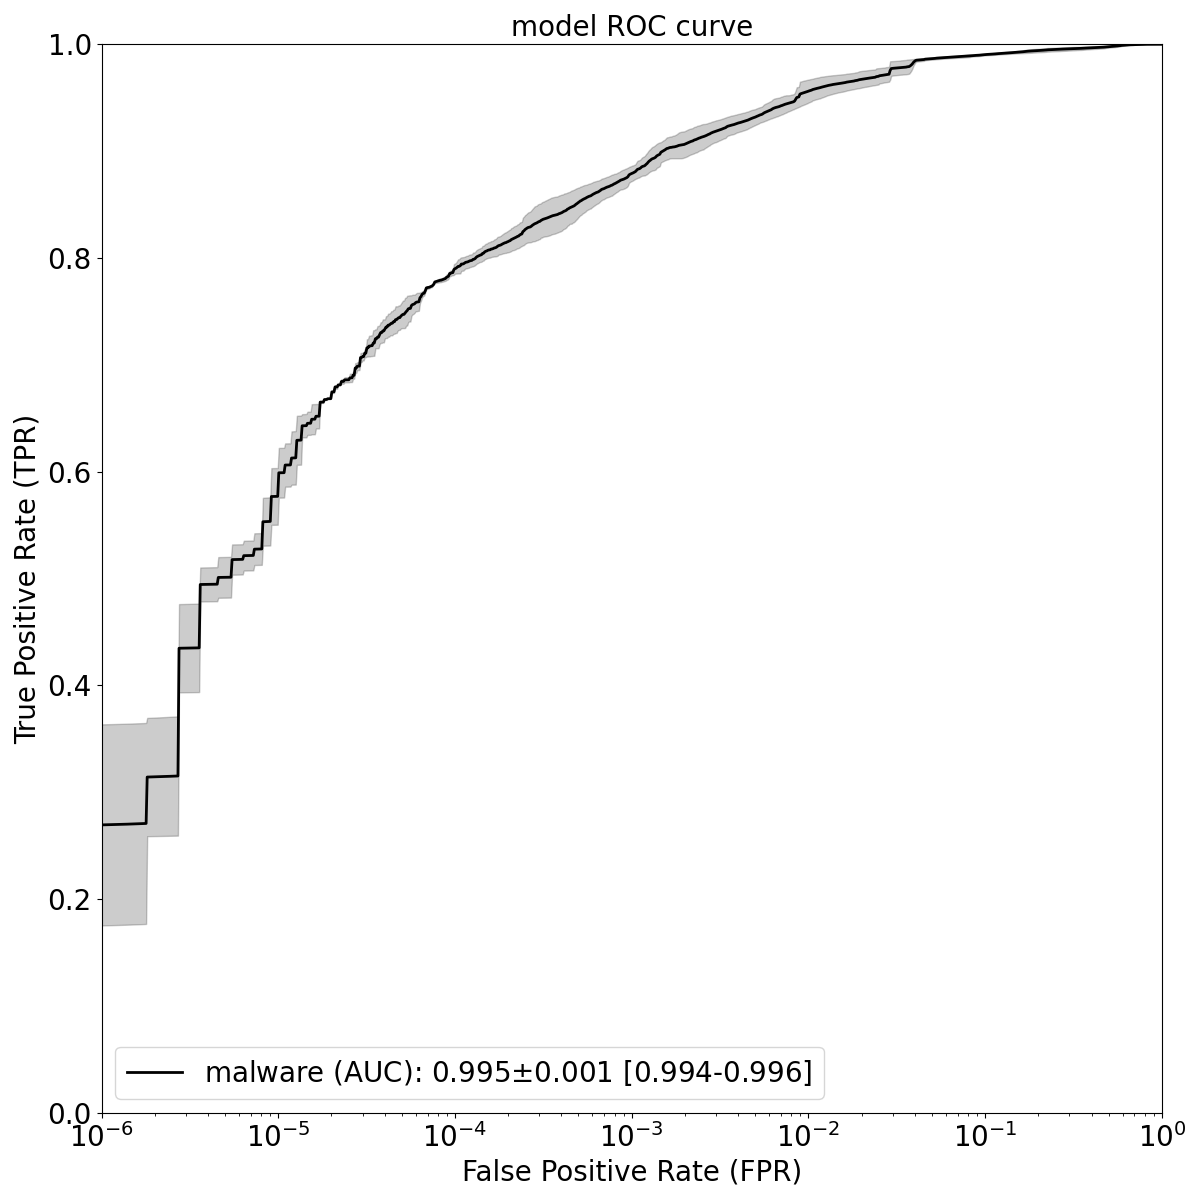
\includegraphics[width=0.8\textwidth]{./results/malware_roc_aloha.png}
		\vspace*{-1cm}
		\caption{Malware ROC ALOHA}
		\label{fig:malwareRocAloha}
	\end{figure}
}

\newcommand{\malwareRocJointEmbedding}{
	\begin{figure}[H]
		\centering
		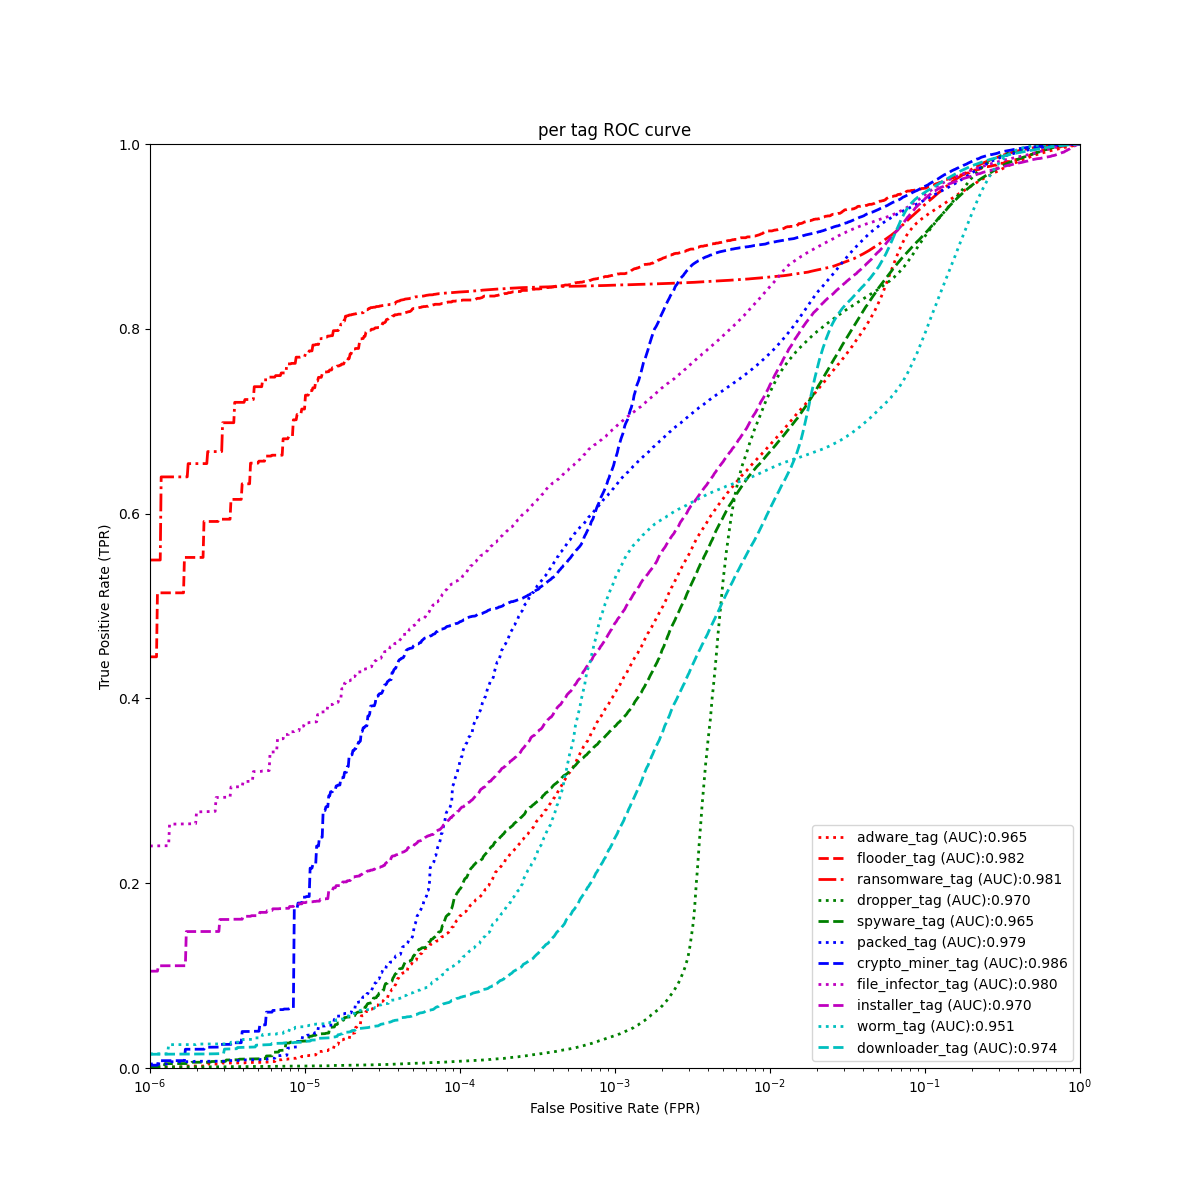
\includegraphics[width=0.8\textwidth]{./results/malware_roc_jointEmbedding.png}
		\vspace*{-1cm}
		\caption{Malware ROC Joint Embedding}
		\label{fig:malwareRocJointEmbedding}
	\end{figure}
}

\newcommand{\malwareRocProposedMethod}{
	\begin{figure}[H]
		\centering
		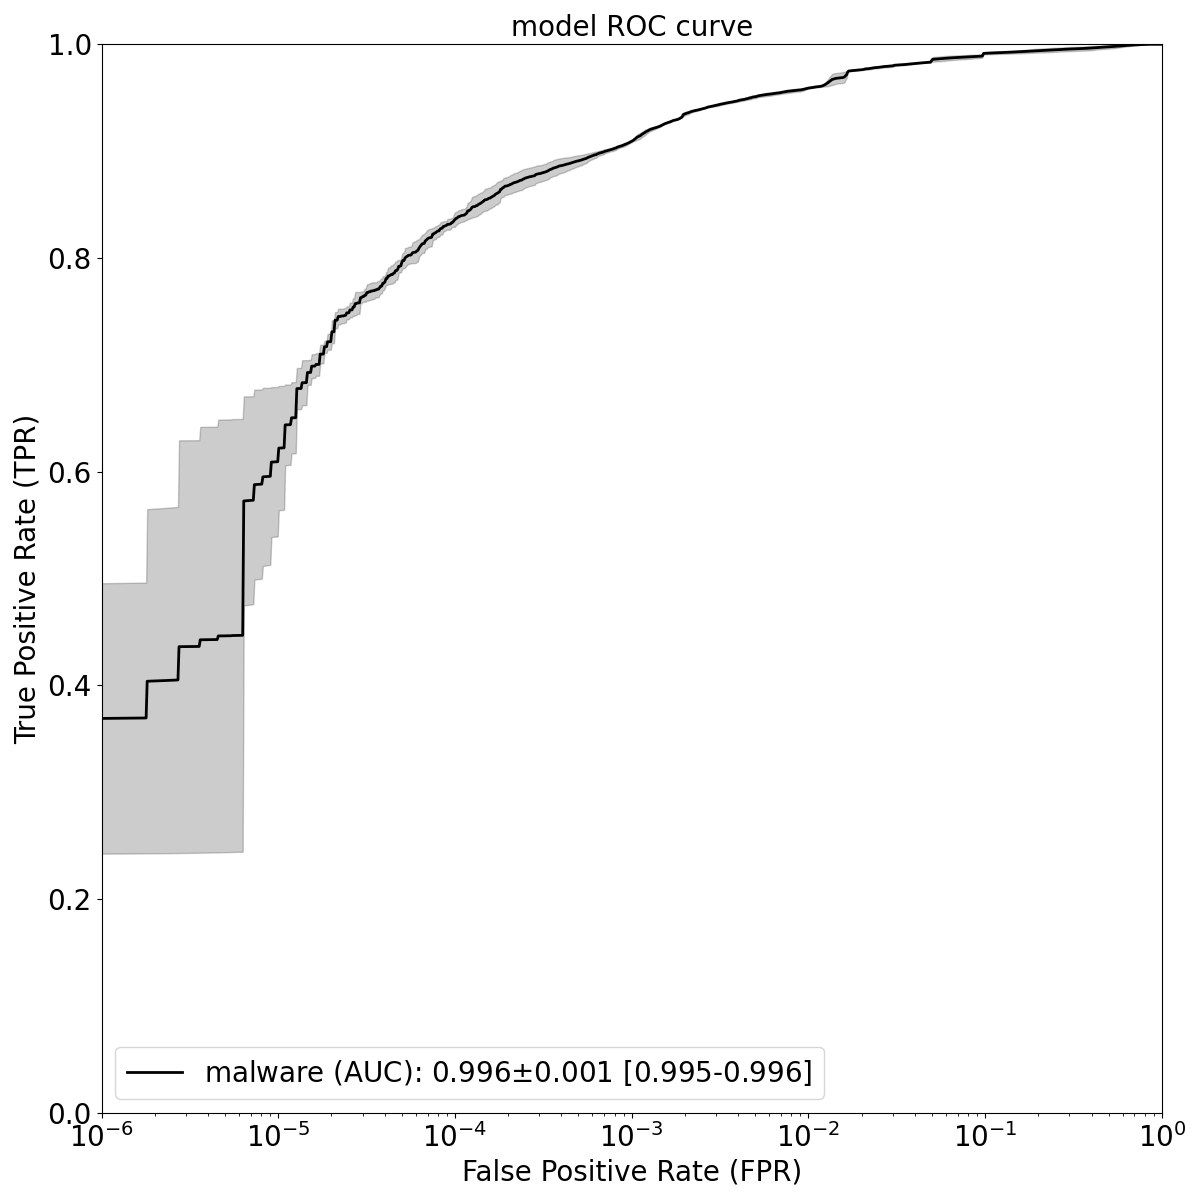
\includegraphics[width=0.8\textwidth]{./results/malware_roc_proposedModel.png}
		\vspace*{-1cm}
		\caption{Malware ROC Proposed Model}
		\label{fig:malawreRocProposedModel}
	\end{figure}
}